%!TEX program = xelatex
%!BIB program = bibtex

\documentclass[en,black,12pt,normal]{elegantpaper}
\usepackage{float}
\usepackage{subfigure}
\usepackage{hyperref}


\newcommand{\upcite}[1]{\textsuperscript{\textsuperscript{\cite{#1}}}}

\title{Bioinformatics Practical Final Report:\\Revisit Aplastic Anemia}
\author{WenYuan Jiang\\ID: 1951510}
\institute{School of Life Science, Tongji University}
%\version{1.00}
\date{\today}
\lstset{basicstyle=\footnotesize\ttfamily,language=R}
\AtBeginEnvironment{lstlisting}{\linespread{0.75}\selectfont}

\begin{document}

\maketitle

\begin{abstract}
\textbf{OBJECTIVE}: We want to demonstrate the skills learnt in this courses by performing a systematical bioinformatics analysis on aplastic anemia. We also aim to reproduce some of the analysis done by previous studies using the same data and similar techniques, and provide insight into this disease.\\
\textbf{RESULTS}: 1) Previous literature suggested a T cell-mediated autoimmune disorder of the hematopoietic system in aplastic anemia patients. 2) Transcriptomics analysis of CD3+ T-cell reveals that platelet factor 4 is related to aplastic anemia pathophysiology. 3) Platelet factor 4 has sequence homology with some chemokine family members. 4) Platelet factor 4 and other CXC chemokine related genes are differently expressed in CD3+ T-cell of aplastic anemia patients. 5) Platelet factor 4 is cleaved into a short form and binds heparin with high affinity. 6) Immunosupressive agent Prednisone has less affinity to PF4, compared with heparin.\\
\textbf{CONCLUSION}: We successfully applied most of what we have learnt in this course to analyse the disease. The analysis indicates that platelet factor 4 in CD3+ cell is related to Aplastic Anemia, and the current immunosupressive treatment of this disease may not affect platelet factor 4 activity directly. 
\keywords{Aplastic Anemia, Review, Bioinformatics, Transcriptomics, Course Final}
\end{abstract}


\tableofcontents

\section{Introduction}

In this paper, we will illustrate the skills we have learned from this course, by applying theories and analytical methods to study a gene named \textbf{MTF-1}.

The paper will first give an overview of MTF-1 and introduce the discovery of MTF-1 gene, which is mostly done in the 1990s by the people working in wet labs. Then, the methods used in this paper will be introduced. Next, results of some analysis using techniques taught in the course will be shown in detail, with steps given in the paper or in supplementary material. Finally, a discussion of the analysis and the results will be presented and we will be talking about issues like the merits and demerits of the methods, what the results indicates and how will these analysis inspire subsequent wet lab works.

Some of the contents of the paper will be based on previous studies, while others will be derived from the data and analysis, which could be inaccurate or misleading. We welcome any kind 
criticism of this paper.

\subsection{Overview of MTF-1}

MTF1 is the metal regulatory transcription factor 1.

In Homo sapiens (human), this gene encodes a transcription factor that induces expression of metallothioneins and other genes involved in metal homeostasis in response to heavy metals such as cadmium, zinc, copper, and silver. The protein is a nucleocytoplasmic shuttling protein that accumulates in the nucleus upon heavy metal exposure and binds to promoters containing a metal-responsive element (MRE).\upcite{ncbi:mtf1human}

\subsection{Discovery of the MTF-1}
In organisms, from the simple prokaryotic cells to complex vertebrate, metals plays an important role since many metal ions are involved in enzymatic reaction. 

The term heavy metal comprises a number of essential and nonessential metals. Among the latter cadmium, mercury and lead are toxic even in trace amounts. Although zinc and copper, which are essential heavy metals, are integral parts of proteins, notably enzymes and transcription factors, an excess of these metals is also toxic. Therefore, elaborate systems to import, sequester, store, transport and expel metals have evolved. Important players in metal homeostasis are the \textbf{metallothioneins}. These small proteins with a high content of cysteines can bind and thereby sequester heavy metals.\upcite{gunther2012taste}

\textbf{Metallothioneins} were discovered in 1957 by Margoshes and Vallee as cadmium-binding proteins in preparations of horse kidney.\upcite{margoshes1957cadmium} Transcription of metallothionein genes is upregulated in response to different stimuli, especially heavy metals. A hallmark of the promoters/enhancers of most metallothionein genes are short DNA sequence motifs termed metal response elements (MREs). The identification of these MREs, that share the core consensus sequence TGCRCNC (R=A or G, N= any nucleotide), suggested the existence of a specific transcription factor that regulates metallothionein expression in response to metals.\upcite{stuart1985identification} In 1988 a MRE-binding protein was identified by electrophoretic mobility shift and methylation interference studies.\upcite{westin1988zinc}\upcite{seguin1988detection} It is bound to its cognate DNA motif in a zinc dependent manner \upcite{westin1988zinc} and was termed MTF-1 (for MRE-binding transcription factor-1, more recently also metal-responsive transcription factor-1 or metal regulatory transcription factor-1). In 1993 the cDNA of mouse MTF-1 was cloned which revealed it as a zinc finger protein.\upcite{radtke1993cloned} Human MTF-1 with a length of 753 amino acids was cloned soon thereafter and found to be highly similar but slightly longer at the C-terminus than mouse MTF-1. \upcite{brugnera1994cloning}\upcite{gunther2012taste}
\section{Materials and Methods}

\subsection{Literature review}

\subsubsection{Source of the literature}
The literature is fetched from PubMed (\url{https://pubmed.ncbi.nlm.nih.gov/})\cite{canese2013pubmed} and PubMed Central (PMC)\cite{roberts2001pubmed}. We searched in PubMed with the key word "acquired aplastic anemia" on \date{\today}. The title, year, abstract is downloaded using the "Save" function on PubMed searching page for further review.

\subsubsection{Word cloud plot}
The word cloud plot is done using \url{https://worditout.com/}. The input data are the selected abstracts of the reviewed articles.

\subsubsection{Selection of the literature}
The selection of the literature is done manually, according to the title and abstract of each article. Our selection standard is shown in the figure below.

\begin{figure}[H]
    \centering
    \includegraphics[width=0.4\textwidth]{image/Classification.png}
    \caption{Selection standard}
    \label{CS}
\end{figure}

\subsection{Transcriptomics analysis (Micro array data)}
\subsubsection{Data source}
The Micro array data used in Transcriptomics analysis is fetched from Gene Expression Omnibus (Gene Expression Omnibus), and the data set will be shown in the Results section.

\subsubsection{Tools and packages}
Transcriptomics analysis is done using R 4.0.5 with the following packages.

\begin{lstlisting}
library(Biobase)
library(GEOquery)
library(limma)
library(umap)
library("FactoMineR")
library("factoextra")
library(pheatmap)
\end{lstlisting}

Quality control of the data, selection of differently expressed genes, principal component analysis and heatmap plotting are done with the packages mentioned above. 

The standard of selection of differently expressed genes is $p\le 0.05$. Among all the differently expressed genes, the top 250 genes are used for principal component analysis and heatmap plotting.

Detailed configuration and code can be found in the Supplementary Material section.

\subsection{GO enrichment analysis}
\subsubsection{Data source}
The data used in GO enrichment analysis is fetched from Gene Expression Omnibus (Gene Expression Omnibus) , and the data set will be shown in the Results section. Annotation data of the GO enrichment comes from the R packages downloaded from Bioconductor\cite{gentleman2004bioconductor}.
\subsubsection{Tools and packages}
Transcriptomics analysis is done using R 4.0.5 with the following packages.

\begin{lstlisting}
library(org.Hs.eg.db)
library(clusterProfiler)
library(dplyr)
\end{lstlisting}

Results are shown in the form of dot plots, with p value and gene ratio labeled on the plot.

Detailed configuration and code can be found in the Supplementary Material section.
\subsection{Sequence analysis}
Sequence analysis is mostly done using online services like BLAST and ConservedDART\cite{geer2002cdart}. While the MSA is done using ClustalX 2.1\cite{larkin2007clustal}.

\subsection{Molecular docking}
The data used for docking is fetched from PDB and ZINC AC\cite{irwin2005zinc} (\url{https://zinc.docking.org/}). We did the molecular docking using the online service swissdock\cite{grosdidier2011swissdock}, with the parameters listed below.
\begin{lstlisting}
JOBNAME: 1PLF_Heparin
EMAIL: 1951510@tongji.edu.cn
PASSIVEFLEXIBILITYDISTANCE: 0.0
WANTEDCONFS: 5000
NBFACTSEVAL: 5000
NBSEEDS: 250
SDSTEPS: 100
ABNRSTEPS: 250
CLUSTERINGRADIUS: 2.0
MAXCLUSTERSIZE: 8
\end{lstlisting}

\subsection{Protein structure visualization}
Protein structure visualization is done using PDB online (Mol* Viewer\cite{sehnal2021mol}) and the visualization of docking results is done by UCSF Chimera\cite{pettersen2004ucsf}.


\section{Results}

\subsection{Previous literature suggested a T cell-mediated autoimmune disorder of the hematopoietic system.}

Among all the 513 search results, there are 43 articles about aplastic anemia involves certain bioinformatics analysis, ranging from sequence comparison to transcriptomics analysis. 

All the 43 articles mentioned autoimmune disorder in most aplastic anemia cases, while 12 of them gives us an insight that T cell-mediated autoimmune disorder is closely related to aplastic anemia. Immune-mediated destruction of hematopoietic stem and progenitor cells is pathophysiologic in most cases of aplastic anemia (AA).\cite{zeng2004transcript}

The generated word cloud plot is shown below.

\begin{figure}[H]
    \centering
    \includegraphics[width=0.6\textwidth]{image/wordcloud.png}
    \caption{Selection standard}
    \label{WORD}
\end{figure}

We selected several articles involving the bioinfomatics skills we have learnt in this course as our data source to perform our analysis. The selected articles are listed in Supplementary Material section.


\subsection{Transcriptomics analysis of CD3+ T-cell reveals that platelet factor 4 is related to aplastic anemia pathophysiology.}

We fetched the data set GSE3807 from GEO. The data set is collected from 8 volunteers using Affymetrix Human Genome U133A Array (GPL96). Among the 8 samples, 6 are suffering from aplastic anemia, while the other 2 samples are from healthy control.\cite{franzke2006identification}

We identified the top 250 differently expressed genes from the data set, with the worst p value of 0.011. Using the differently expressed genes, we did a principal component analysis, and the result is shown below.

\begin{figure}[H]
    \centering
    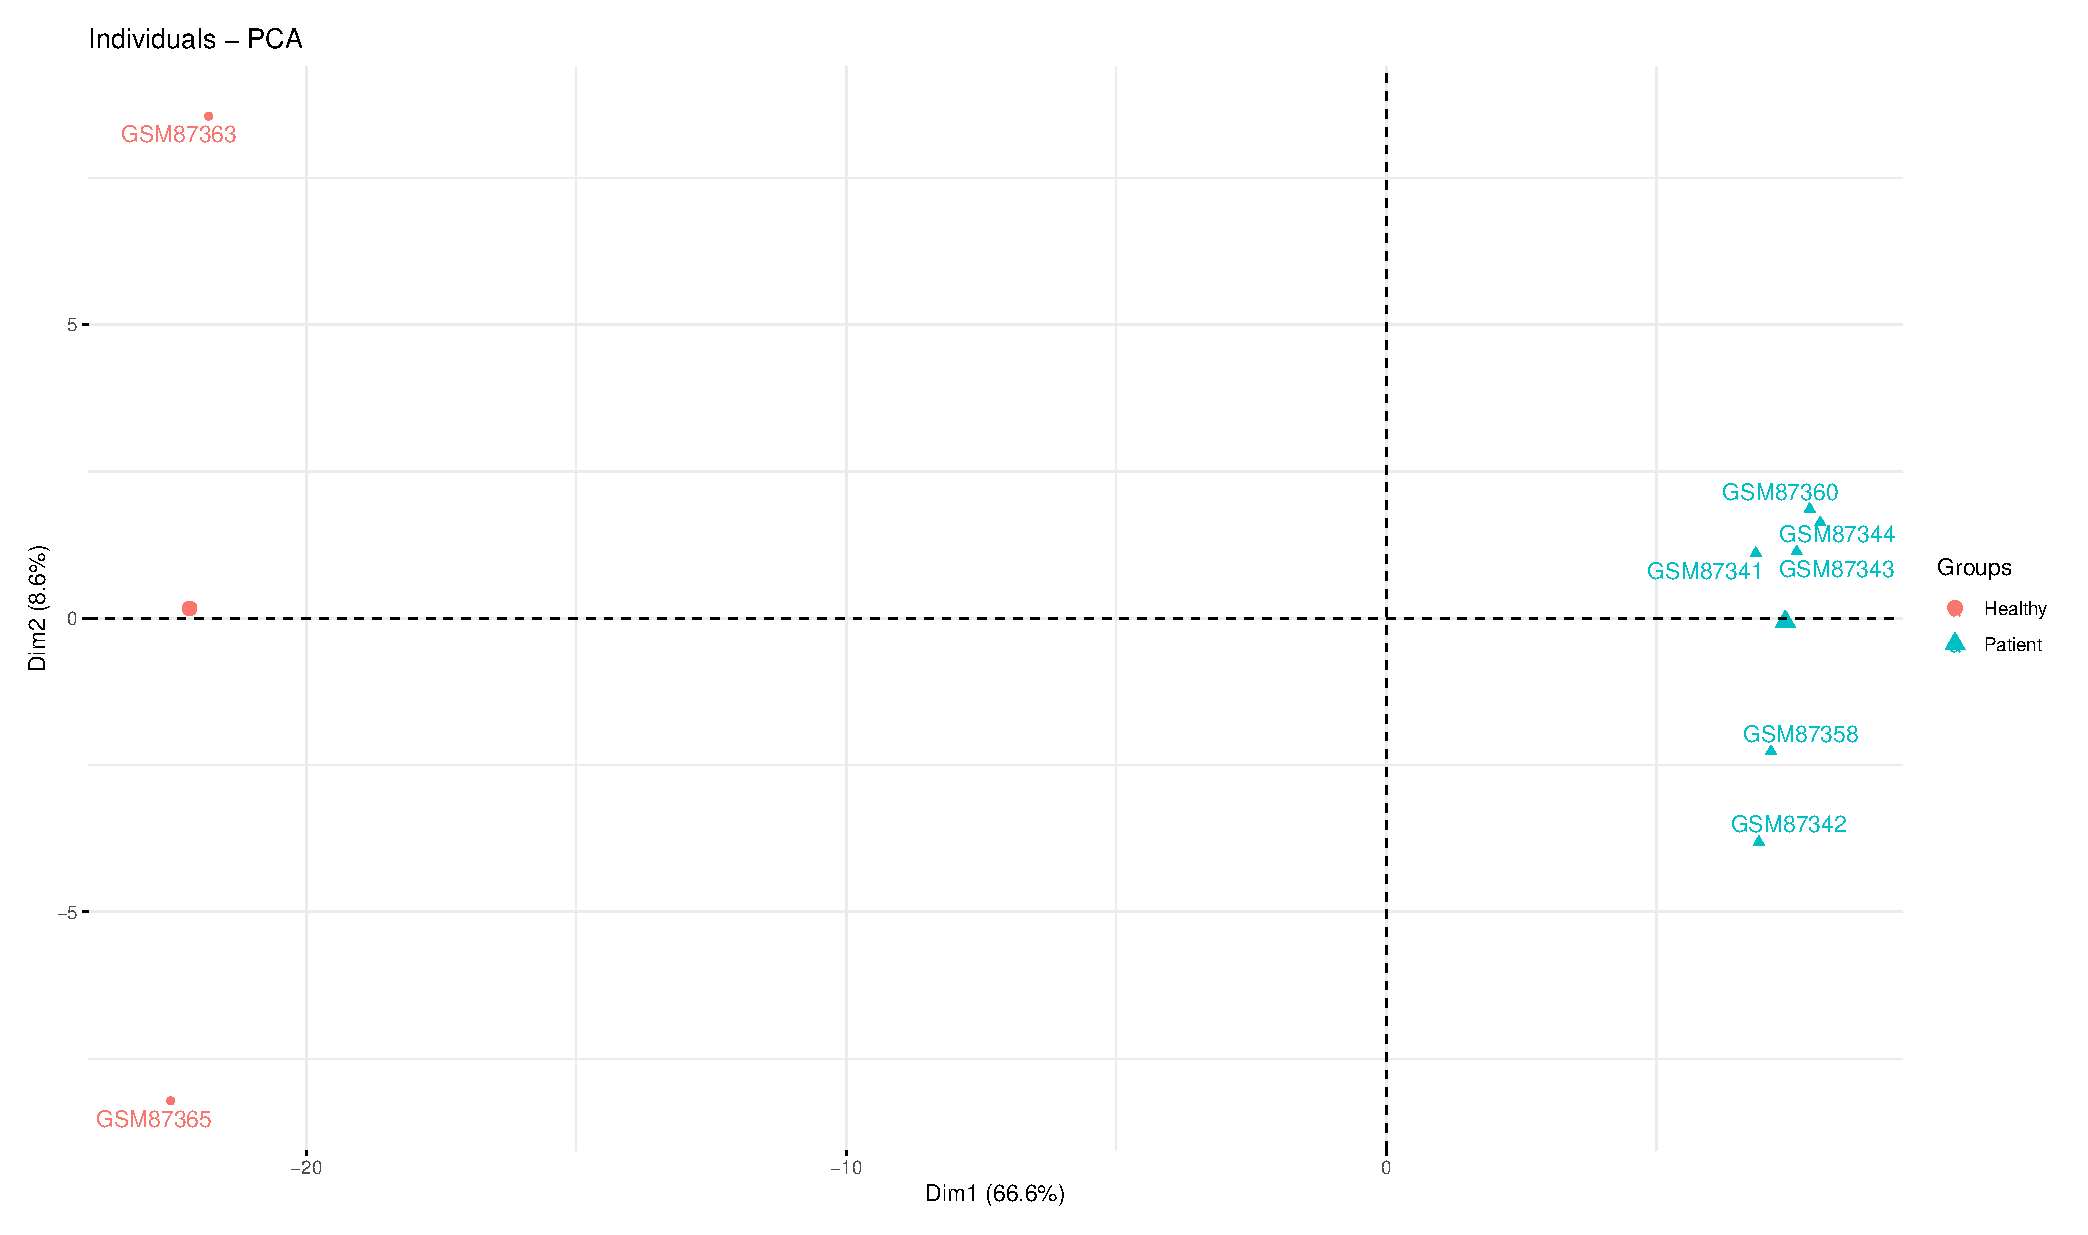
\includegraphics[width=0.9\textwidth]{image/PCACD31.eps}
    \caption{Result of principal component analysis}
    \label{PCACD3}
\end{figure}

PC1 and PC2 consist over 70\% of the principal components, which indicates that the analysis is desirable. According to the figure above, two groups of people are well separated by the PC1 and PC2 of the principal component analysis algorithm.

\begin{figure}[H]
    \centering
    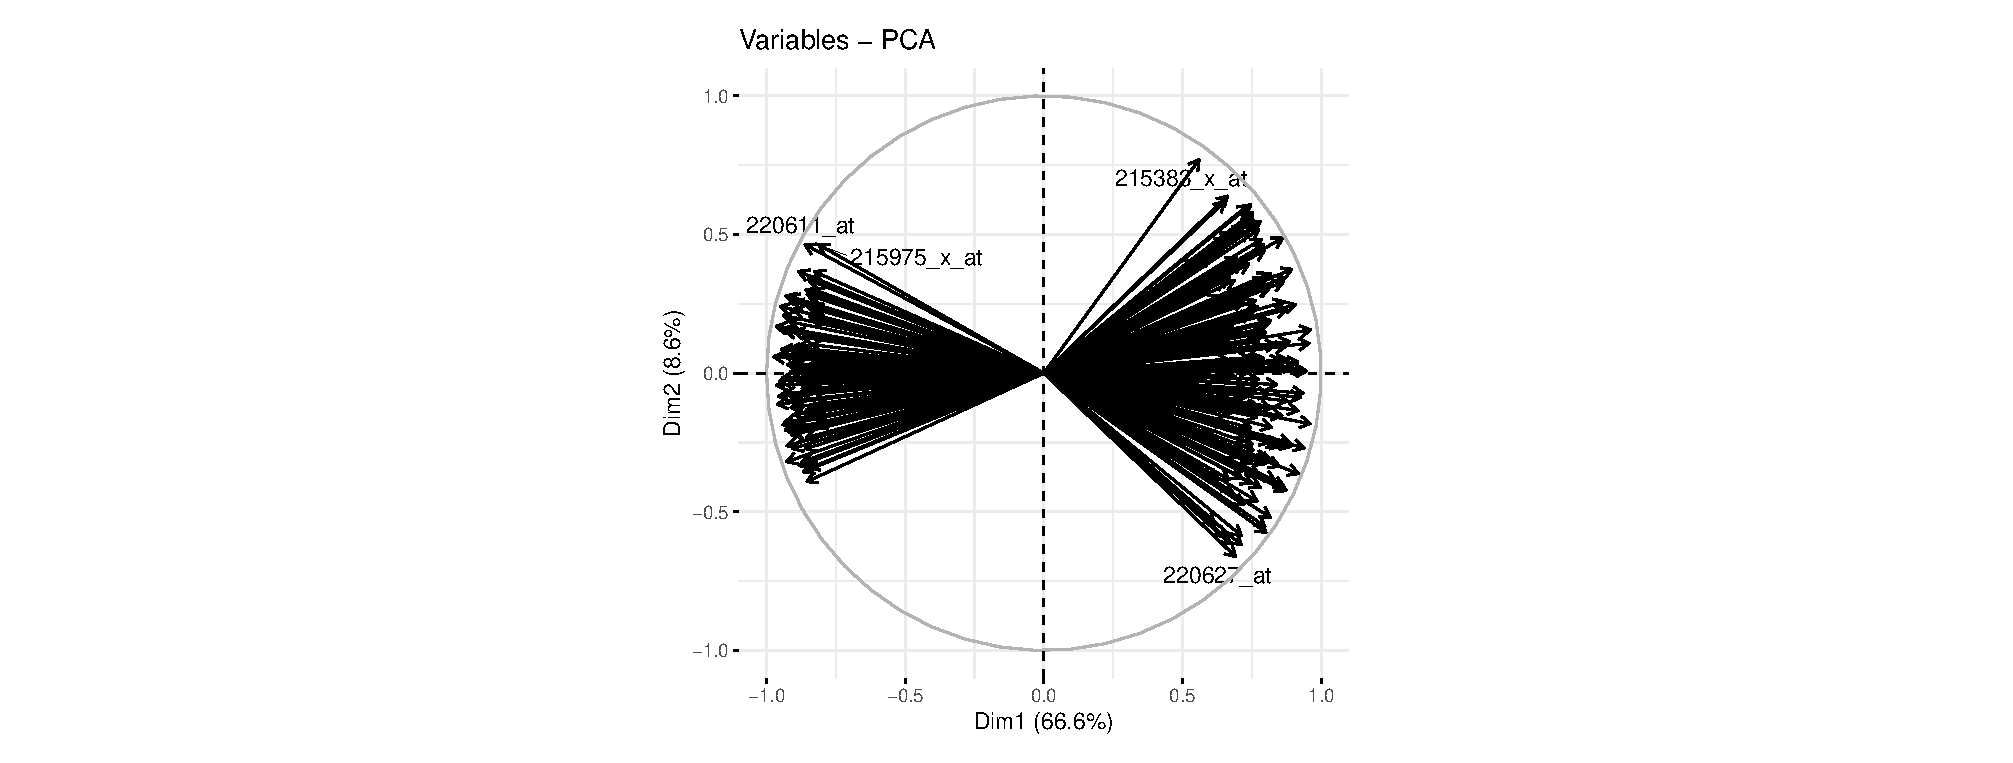
\includegraphics[width=0.5\textwidth]{image/PCAVCD3.eps}
    \caption{Variance of principal component analysis}
    \label{PCACD3}
\end{figure}


Heat map of the differently expressed genes is shown below.

\begin{figure}[H]
    \centering
    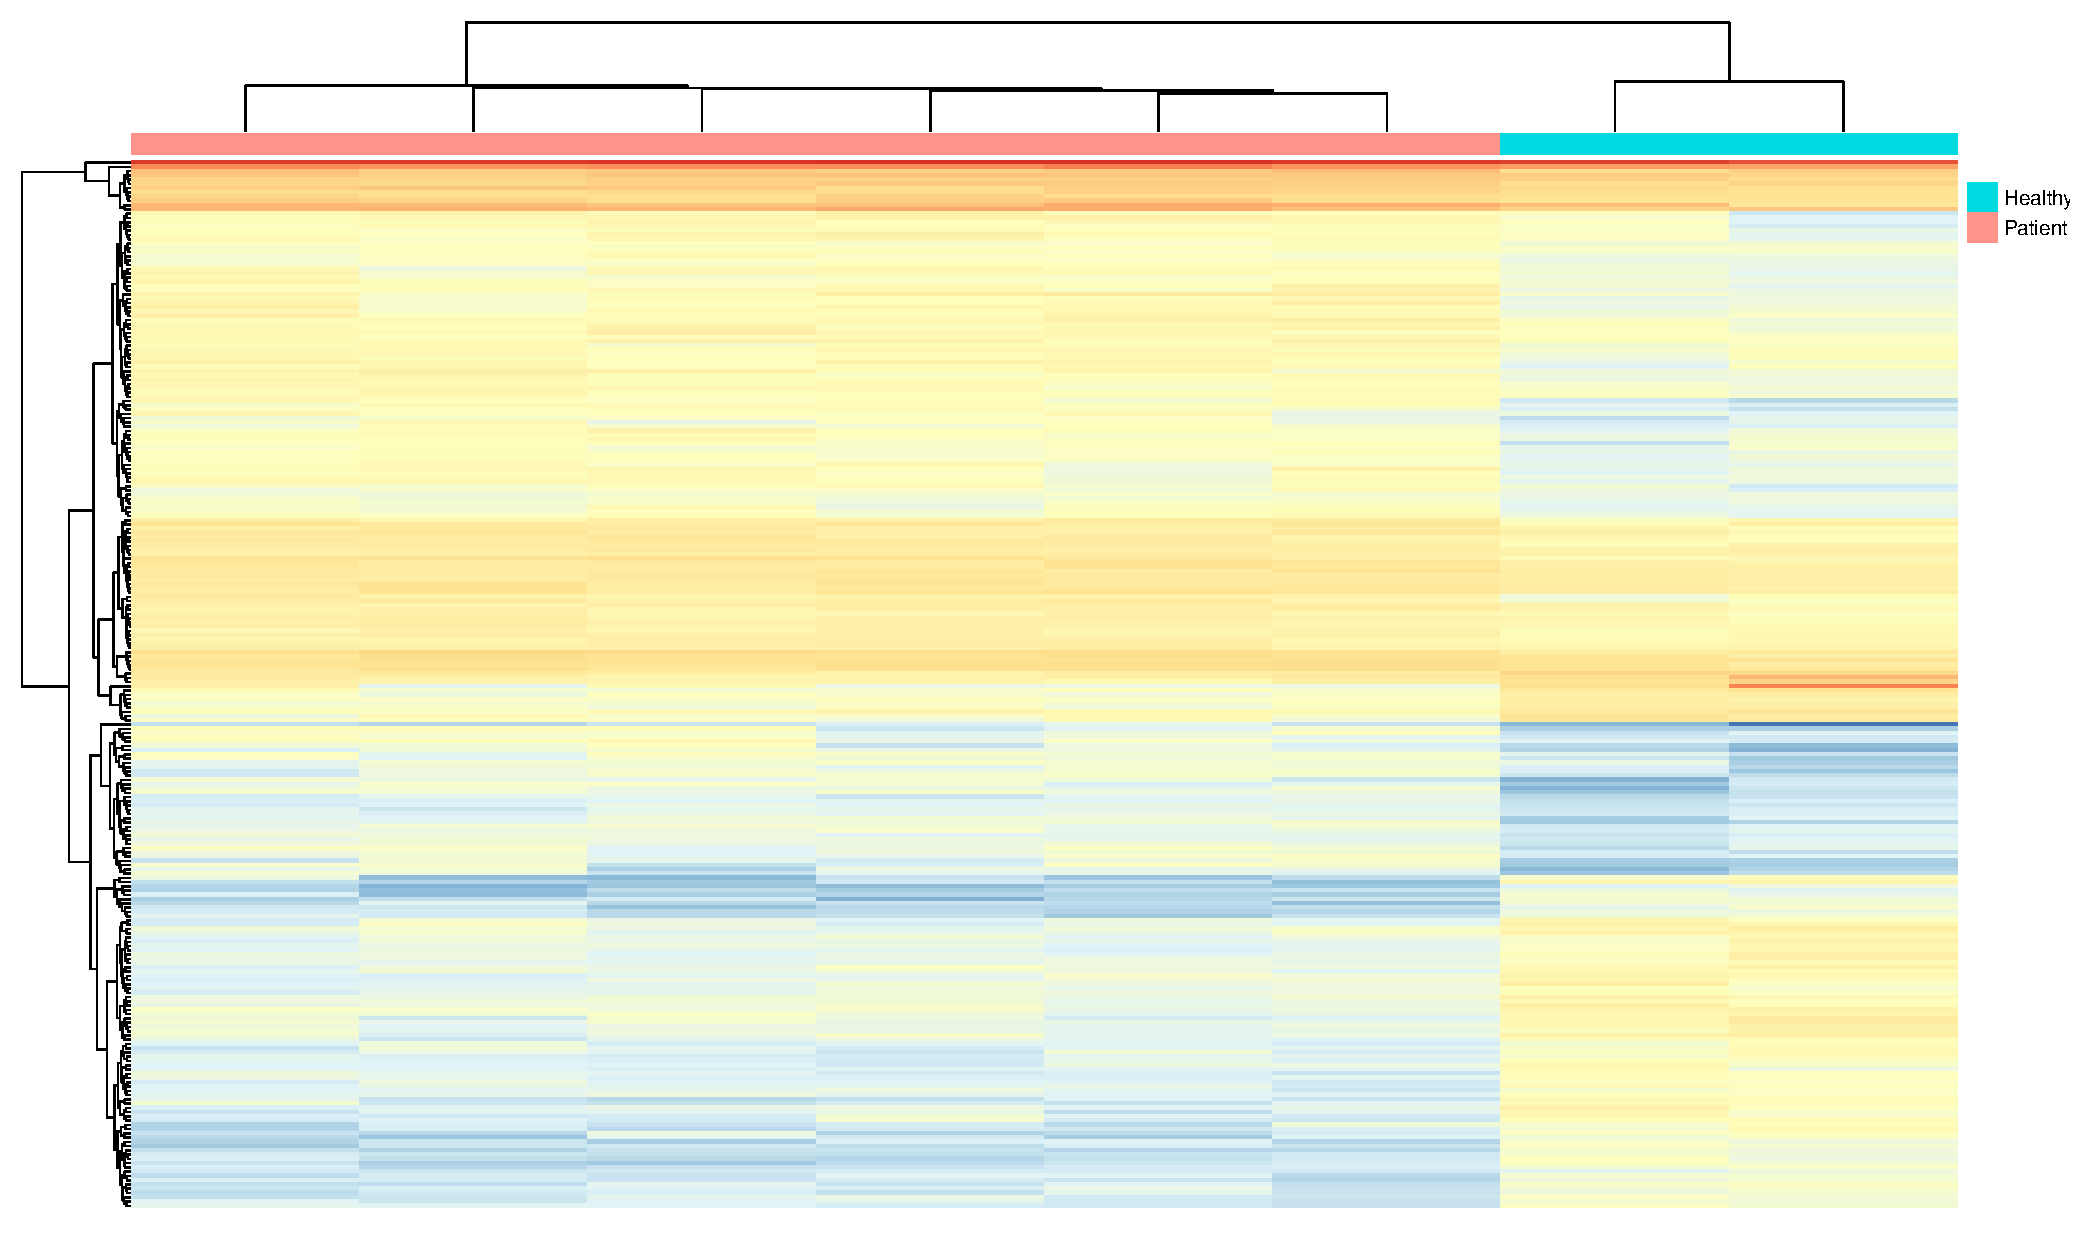
\includegraphics[width=0.9\textwidth]{image/HMCD3.eps}
    \caption{Heat map of the differently expressed genes}
    \label{HMCD3}
\end{figure}

From the heat map and the clustering results, clear divergence can be seen between the two groups. The main difference of the two groups are the genes that are down regulated in the Patients group, which is the lower-left part of the heat map.

To find out the functions of the down regulated genes, we did a GO enrichment on all down regulated genes, and the resulting dot plot is shown below.

\begin{figure}[H]
    \centering
    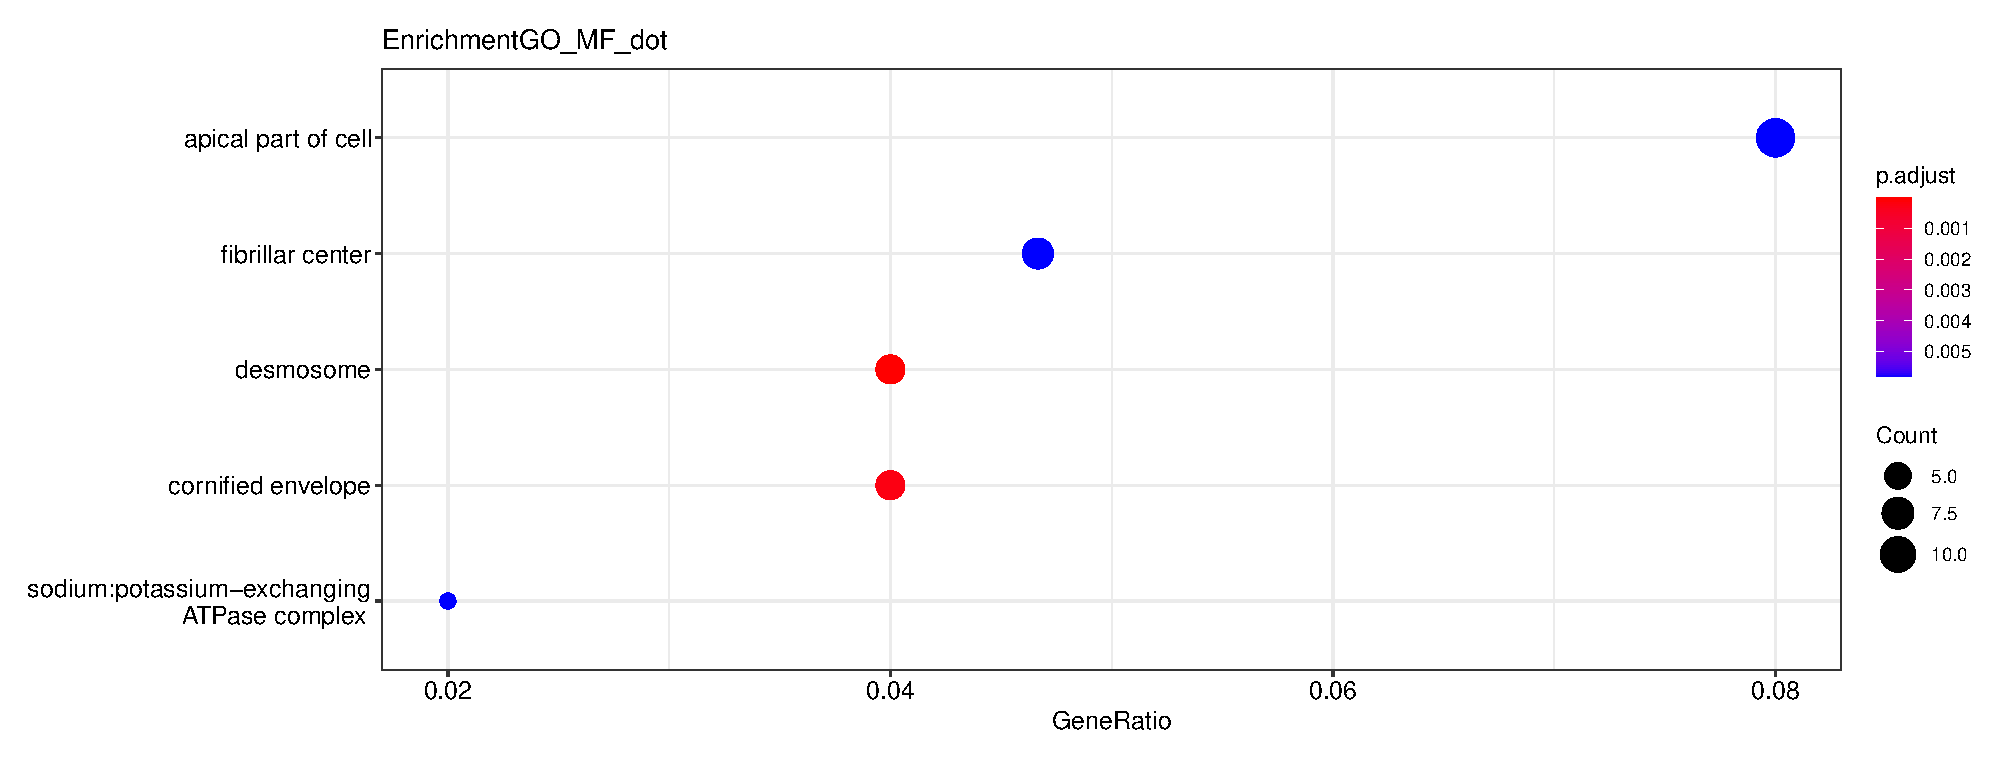
\includegraphics[width=1\textwidth]{image/EGOCD3.eps}
    \caption{GO enrichment of down regulated genes}
    \label{HMCD3}
\end{figure}

Among the down regulated genes, one gene named platelet factor 4 (PF4) caught our attention. PF4 is 27 folds lower in the patients group than in healthy control, and the p value of the gene is 0.005. Considering that PF4 is closely related to platelet formation and functions, we can say that platelet factor 4 is related to aplastic anemia pathophysiology.

\subsection{Platelet factor 4 has sequence homology with some chemokine family members.}

We fetched the sequence of Platelet factor 4, and run a psi-blast against the NCBI protein database, and the organism is limited to human. The results are then analysed using ClustalX 2.1 to perform an MSA.

\begin{figure}[H]
    \centering
    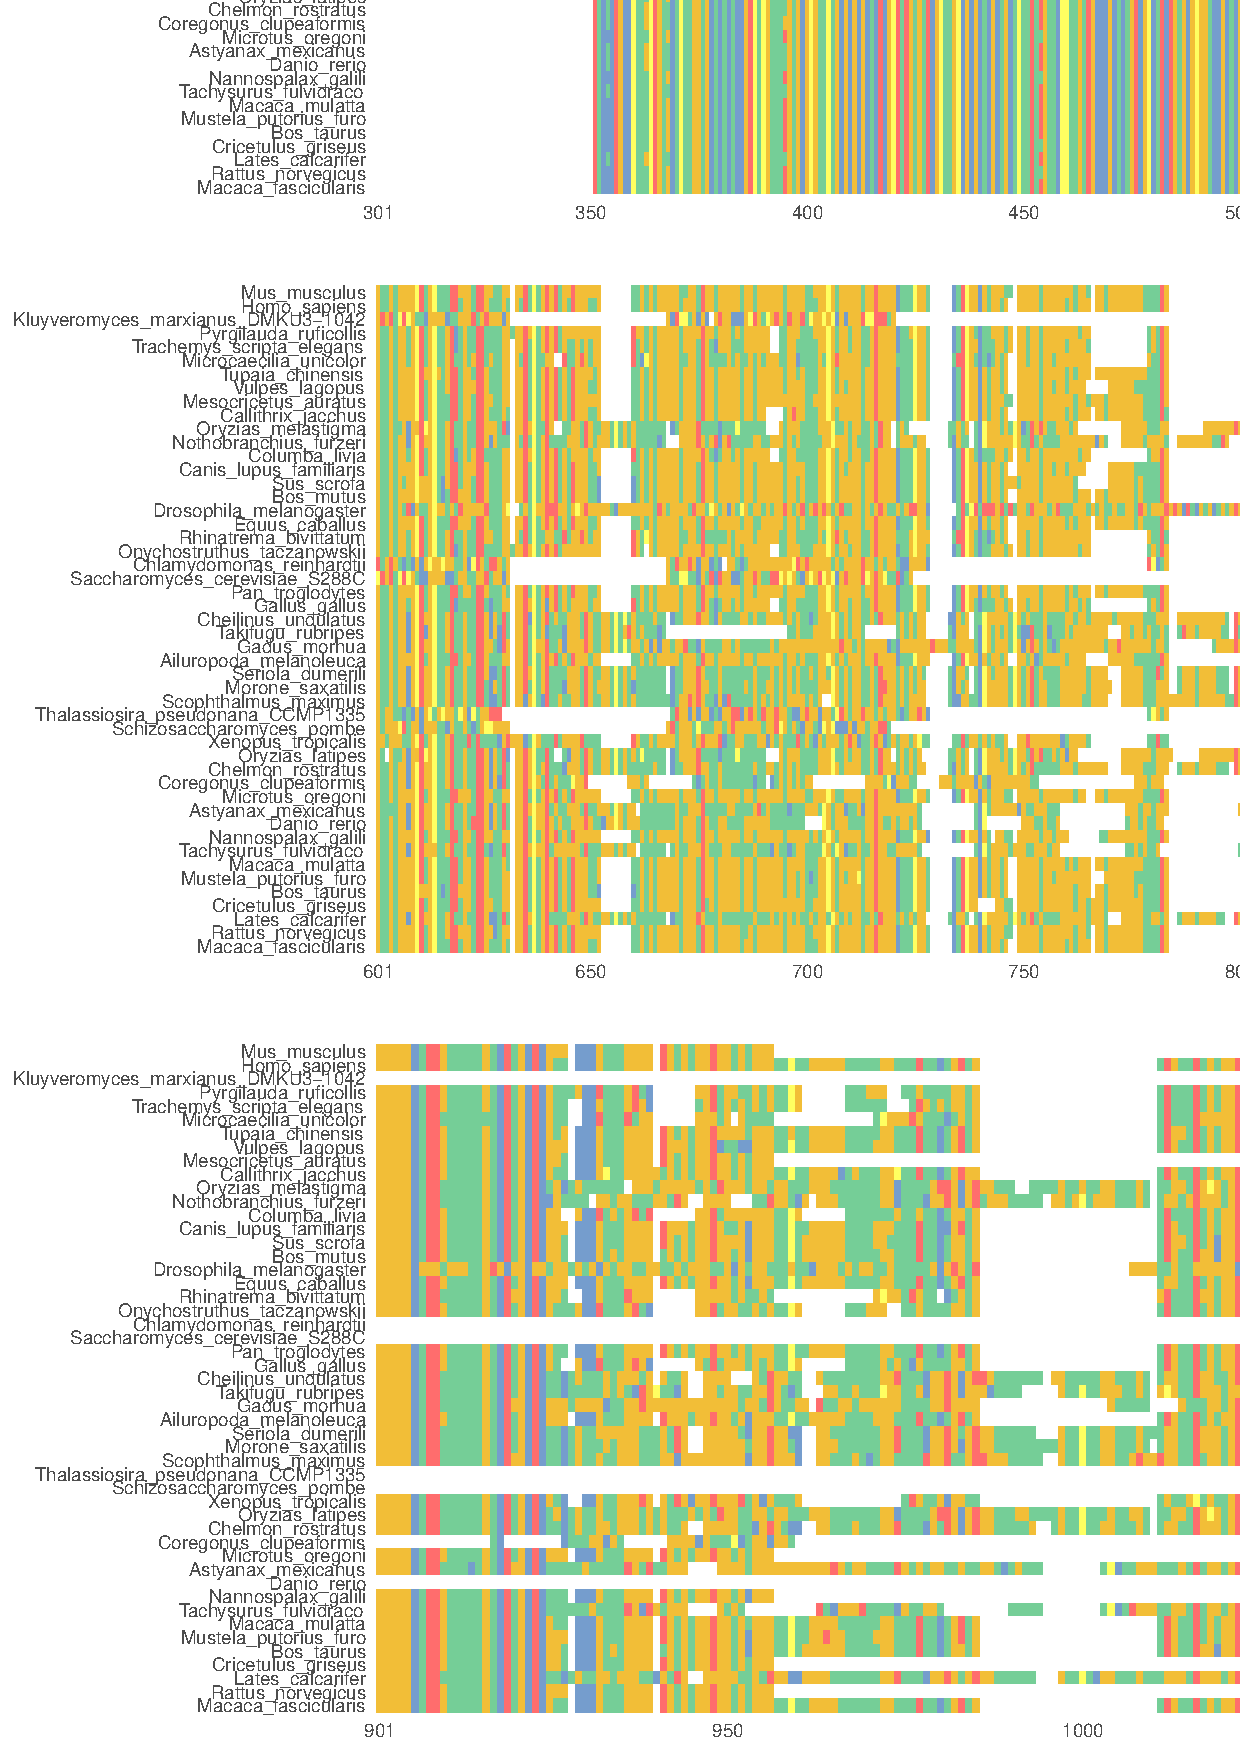
\includegraphics[width=1\textwidth]{image/MSA.png}
    \caption{MSA results}
    \label{HMCD3}
\end{figure}

According to the MSA results, A consensus pattern named C-X-C motif can be found in PF4 (NP\_002611.1). The hits indicated a conserved domain that classifies the PF4 into CXC family chemokine, which is a chemotactic factor that attracts neutrophils, basophils, and T-cells, but not monocytes, and is involved in neutrophil activation.

\begin{figure}[H]
    \centering
    \includegraphics[width=1\textwidth]{image/PF4D.png}
    \caption{Conserved domain of Platelet factor 4}
    \label{HMCD3}
\end{figure}

Visualization of the PF4 is shown in the figure below. The purple colored part is the C-X-C motif.

\begin{figure}[H]
    \centering
    \includegraphics[width=1\textwidth]{image/PF43D2.png}
    \caption{Structure and Conserved domain of Platelet factor 4}
    \label{HMCD3}
\end{figure}

According to previous literature, platelet factor 4 (PF4) is a small cytokine belonging to the CXC chemokine family that is also known as chemokine (C-X-C motif) ligand 4 (CXCL4). This chemokine is released from alpha-granules of activated platelets during platelet aggregation, and promotes blood coagulation by moderating the effects of heparin-like molecules. Due to these roles, it is predicted to play a role in wound repair and inflammation. It is usually found in a complex with proteoglycan.\cite{fernandez2002structure}

\subsection{Platelet factor 4 and other CXC chemokine related genes are differently expressed in CD3+ T-cell of aplastic anemia patients.}

Among all the genes that are related to CXC chemokine family, 34 of them are measured on the micro array. There are 24 of the 34 relevant genes are down regulated in the patient group compared with the healthy control, while others are slightly up regulated. The differently expressed CXC chemokine related genes and their logFC values are demonstrated in the heat map below.

\begin{figure}[H]
    \centering
    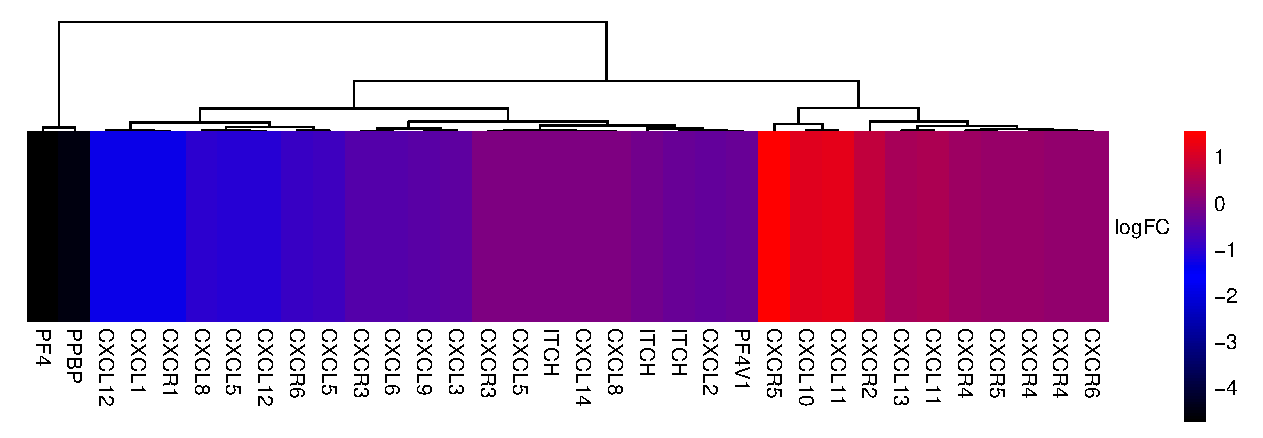
\includegraphics[width=1\textwidth]{image/CXCHM.eps}
    \caption{Structure and Conserved domain of Platelet factor 4}
    \label{HMCD3}
\end{figure}

\subsection{Platelet factor 4 is cleaved into a short form and binds heparin with high affinity.}

We queried the Nextprot database for more detailed information about Platelet factor 4. The platelet factor 4 has its signal peptide cut to form the mature protein, and the mature protein is cleaved into a short form, which can bind strongly to heparin. The figure below shows the sequence features of Platelet factor 4.

\begin{figure}[H]
    \centering
    \includegraphics[width=1\textwidth]{image/PF4ISO.png}
    \caption{Sequence features of Platelet factor 4}
    \label{HMCD3}
\end{figure}

According to the GO annotation of platelet factor 4 in the database, it has high affinity to bind heparin, and we did a molecular docking to confirm this claim \textit{in silico}. 

The lowest energy conformation is shown in the figure below.

\begin{figure}[H]
    \centering
    \includegraphics[width=0.7\textwidth]{image/DOCK.png}
    \caption{Lowest energy docking conformation}
    \label{HMCD3}
\end{figure}

\begin{lstlisting}
REMARK  Energy: -17.5306
REMARK  SimpleFitness: -17.5306
REMARK  FullFitness: -2058.942
REMARK  InterFull: -308.048
REMARK  IntraFull: 42.5802
REMARK  solvFull: -1990.93
REMARK  surfFull: 197.456
REMARK  extraFull: 0.0
REMARK  deltaGcompsolvpol: -1990.93
REMARK  deltaGcompsolvnonpol: 197.456
REMARK  deltaGprotsolvpol: -2104.32
REMARK  deltaGprotsolvnonpol: 195.666
REMARK  deltaGligsolvpol: -171.412
REMARK  deltaGligsolvnonpol: 12.8132
REMARK  deltaGvdw: -308.048
REMARK  deltaGelec: 0.0
REMARK  deltaG: -16.744253
REMARK  Cluster: 0
REMARK  ClusterRank: 0
\end{lstlisting}





\subsection{Immunosupressive agent Prednisone has less affinity to PF4, compared with heparin.}

We also docked commonly used immunosupressive agents like Prednisone, Cyclosporin and Tacrolimus, which are used in immunosupressive therapies, but they showed little affinity to PF4, compared with heparin.

The docking result of Prednisone is shown below.

\begin{figure}[H]
    \centering
    \includegraphics[width=0.7\textwidth]{image/DOCK2.png}
    \caption{Lowest energy docking conformation}
    \label{HMCD3}
\end{figure}

\begin{lstlisting}
REMARK  Energy: 26.0314
REMARK  SimpleFitness: 26.0314
REMARK  FullFitness: -1853.696
REMARK  InterFull: -36.5928
REMARK  IntraFull: 81.3677
REMARK  solvFull: -2095.95
REMARK  surfFull: 197.479
REMARK  extraFull: 0.0
REMARK  deltaGcompsolvpol: -2095.95
REMARK  deltaGcompsolvnonpol: 197.479
REMARK  deltaGprotsolvpol: -2104.32
REMARK  deltaGprotsolvnonpol: 195.666
REMARK  deltaGligsolvpol: -17.0954
REMARK  deltaGligsolvnonpol: 11.6588
REMARK  deltaGvdw: -36.5928
REMARK  deltaGelec: 0.0
REMARK  deltaG: -6.8246017
REMARK  Cluster: 0
REMARK  ClusterRank: 0

\end{lstlisting}

The optimal conformation in the figure above has -6.82 Estimated $\delta$G (kcal/mol) which is relatively weak. This indicates that Prednisone as an immunosupressive agent, may not be directly affecting the function of PF4.

\section{Discussion \& Conclusions}

We started our analysis from the multiple sequence alignment of MTF-1 protein sequence in different organisms and find out that protein sequence of MTF-1 is conserved in different organisms. We then analysed the nucleotide sequence of MTF-1, and found that the exon and intron patterns share a high similarity among these organisms.

Similar sequence indicates that similar feathers and functions exist. Therefore we did analysis on the physicochemical properties of MTF-1 in in different organisms, and the results are consistent with our initial guess.

To study the function of MTF-1, we first checked the sequence for special domains. Nuclear localization signal and Zinc finger domain are found, which suggests that MTF-1 works like a transcription factor. Since the zinc finger domains can recognize and bind to specific DNA sequences, we would like to know what the target sequences are. Fortunately, suitable tools are published and we are able to get the consensus sequence of MTF-1 target/binding sequences.

With the MTF-1 target/binding sequences, the question about what genes are regulated via the MTF-1 target/binding sequences (that is, metal response elements MREs) formed. Through sequence screening and transcriptome analysis, several genes that are likely to be regulated by MTF-1 is found.

Still, we do not know the exact structure of the MTF-1, since homologous modeling of MTF-1 fails to give out reasonable structures. \textit{Ab initio} methods, however, cost too much time and computation resources for facilities to afford. Considering that MTF-1 is an unstable protein, elucidation opf its structure by X-ray crystallography may face difficulties, and other methods, like NMR, is not suitable for such a large protein. Cryoelectron Microscopy might be a choice for this task, butin our literature review, no relevant work was found.

If we have the exact structure of the MTF-1, many processes involving MTF-1 will be studied more deeply, and we can gain more insight into the mechanisms of metal regulatory transcription factor, including but not limited to MTF-1.
\section{Conclusions}
In this report, we successfully applied most of what we have learnt in this course to perform a systematical bioinformatics analysis on the disease Aplastic Anemia. The analysis we have done indicates that platelet factor 4 in CD3+ cell is related to Aplastic Anemia, and the reasons behind the regulation of platelet factor 4 expression can be of significance to the treatment of this disease. Moreover, immunosupressive agent Prednisone may not directly influence the function of PF4, which suggests that current immunosupressive threapy might be safe to some extent. Since 1900s, we humans have begun to study this threatening disease, but till now, the molecular mechanism of this disease still remains unclear, and there is no effective treatment to Aplastic Anemia. 

However, due to limited access to literature, first-hand data and hardware resources, some analysis could not be done, such as the analysis of deep sequencing data, metabolomics study, SNP detection of certain genes in patients' T-cells, analysis of beta chain variability of T-cell receptor and etc.

We hope that our analysis can give future researchers guidance and insight into the mechanism behind this disease, and we believe that bioinformatics will play a more important role in the study of all types of diseases.
\section*{Acknowledgment}

Throughout the writing of this report I have received a great deal of support and assistance.

I would like to thank the teachers of the course, whose expertise was invaluable in formulating the research questions and methodology. 

I would also like to acknowledge my classmates in this course for their wonderful collaboration. I would particularly like to single out Zhifan Lin, I want to thank you for your patient support and insightful suggestions.
\section*{Supplementary Materials}

\subsection*{Literature used as data source}
\begin{itemize}
    \item Franzke A, Geffers R, Hunger JK, Pförtner S et al. Identification of novel regulators in T-cell differentiation of aplastic anemia patients. BMC Genomics 2006 Oct 19;7:263. PMID: 17052335
    \item Doi T. [Transcription factors responsible for megakaryocyte-specific gene expression]. Yakugaku Zasshi. 2005 Sep;125(9):685-97. Japanese. doi: 10.1248/yakushi.125.685. PMID: 16141689.
    \item Okada Y, Watanabe M, Nakai T, Kamikawa Y, Shimizu M, Fukuhara Y, Yonekura M, Matsuura E, Hoshika Y, Nagai R, Aird WC, Doi T. RUNX1, but not its familial platelet disorder mutants, synergistically activates PF4 gene expression in combination with ETS family proteins. J Thromb Haemost. 2013 Sep;11(9):1742-50. doi: 10.1111/jth.12355. PMID: 23848403.
\end{itemize}

\subsection*{Computing envrionment}
\begin{lstlisting}
> sessionInfo()
R version 4.0.5 (2021-03-31)
Platform: x86_64-pc-linux-gnu (64-bit)
Running under: Ubuntu 20.04.2 LTS

Matrix products: default
BLAS/LAPACK: /usr/lib/x86_64-linux-gnu/openblas-pthread/libopenblasp-r0.3.8.so

locale:
 [1] LC_CTYPE=en_US.UTF-8       LC_NUMERIC=C              
 [3] LC_TIME=en_US.UTF-8        LC_COLLATE=en_US.UTF-8    
 [5] LC_MONETARY=en_US.UTF-8    LC_MESSAGES=C             
 [7] LC_PAPER=en_US.UTF-8       LC_NAME=C                 
 [9] LC_ADDRESS=C               LC_TELEPHONE=C            
[11] LC_MEASUREMENT=en_US.UTF-8 LC_IDENTIFICATION=C       

attached base packages:
 [1] stats4    grid      parallel  stats     graphics 
 [6] grDevices utils     datasets  methods   base     

other attached packages:
 [1] pathview_1.30.1        clusterProfiler_3.18.1
 [3] topGO_2.42.0           SparseM_1.81          
 [5] GO.db_3.12.1           graph_1.68.0          
 [7] org.Hs.eg.db_3.12.0    AnnotationDbi_1.52.0  
 [9] IRanges_2.24.1         S4Vectors_0.28.1      
[11] DOSE_3.16.0            maptools_1.1-1        
[13] sp_1.4-5               factoextra_1.0.7      
[15] ggplot2_3.3.3          FactoMineR_2.4        
[17] VennDiagram_1.6.20     futile.logger_1.4.3   
[19] pheatmap_1.0.12        umap_0.2.7.0          
[21] limma_3.46.0           GEOquery_2.58.0       
[23] Biobase_2.50.0         BiocGenerics_0.36.1   

loaded via a namespace (and not attached):
  [1] readxl_1.3.1         shadowtext_0.0.8    
  [3] backports_1.2.1      fastmatch_1.1-0     
  [5] plyr_1.8.6           igraph_1.2.6        
  [7] splines_4.0.5        BiocParallel_1.24.1 
  [9] digest_0.6.27        htmltools_0.5.1.1   
 [11] GOSemSim_2.16.1      viridis_0.6.1       
 [13] fansi_0.5.0          magrittr_2.0.1      
 [15] memoise_2.0.0        cluster_2.1.1       
 [17] openxlsx_4.2.3       Biostrings_2.58.0   
 [19] readr_1.4.0          graphlayouts_0.7.1  
 [21] matrixStats_0.59.0   askpass_1.1         
 [23] enrichplot_1.10.2    colorspace_2.0-1    
 [25] blob_1.2.1           ggrepel_0.9.1       
 [27] haven_2.4.1          xfun_0.23           
 [29] dplyr_1.0.6          RCurl_1.98-1.3      
 [31] crayon_1.4.1         jsonlite_1.7.2      
 [33] scatterpie_0.1.6     glue_1.4.2          
 [35] polyclip_1.10-0      gtable_0.3.0        
 [37] zlibbioc_1.36.0      XVector_0.30.0      
 [39] car_3.0-10           Rgraphviz_2.34.0    
 [41] abind_1.4-5          scales_1.1.1        
 [43] futile.options_1.0.1 DBI_1.1.1           
 [45] rstatix_0.7.0        Rcpp_1.0.6          
 [47] viridisLite_0.4.0    reticulate_1.20     
 [49] flashClust_1.01-2    foreign_0.8-81      
 [51] bit_4.0.4            DT_0.18             
 [53] httr_1.4.2           htmlwidgets_1.5.3   
 [55] fgsea_1.16.0         RColorBrewer_1.1-2  
 [57] ellipsis_0.3.2       XML_3.99-0.6        
 [59] pkgconfig_2.0.3      farver_2.1.0        
 [61] utf8_1.2.1           tidyselect_1.1.1    
 [63] labeling_0.4.2       rlang_0.4.11        
 [65] reshape2_1.4.4       munsell_0.5.0       
 [67] cellranger_1.1.0     tools_4.0.5         
 [69] cachem_1.0.5         downloader_0.4      
 [71] cli_2.5.0            generics_0.1.0      
 [73] RSQLite_2.2.7        broom_0.7.6         
 [75] stringr_1.4.0        fastmap_1.1.0       
 [77] bit64_4.0.5          tidygraph_1.2.0     
 [79] zip_2.2.0            purrr_0.3.4         
 [81] KEGGREST_1.30.1      ggraph_2.0.5        
 [83] formatR_1.11         KEGGgraph_1.50.0    
 [85] DO.db_2.9            leaps_3.1           
 [87] xml2_1.3.2           compiler_4.0.5      
 [89] rstudioapi_0.13      curl_4.3.1          
 [91] png_0.1-7            ggsignif_0.6.1      
 [93] tibble_3.1.2         tweenr_1.0.2        
 [95] stringi_1.6.2        RSpectra_0.16-0     
 [97] forcats_0.5.1        lattice_0.20-41     
 [99] Matrix_1.3-2         vctrs_0.3.8         
[101] pillar_1.6.1         lifecycle_1.0.0     
[103] BiocManager_1.30.15  bitops_1.0-7        
[105] data.table_1.14.0    cowplot_1.1.1       
[107] qvalue_2.22.0        R6_2.5.0            
[109] gridExtra_2.3        rio_0.5.26          
[111] lambda.r_1.2.4       MASS_7.3-53.1       
[113] assertthat_0.2.1     openssl_1.4.4       
[115] withr_2.4.2          hms_1.1.0           
[117] tidyr_1.1.3          rvcheck_0.1.8       
[119] carData_3.0-4        ggpubr_0.4.0        
[121] ggforce_0.3.3        scatterplot3d_0.3-41
[123] tinytex_0.32        
\end{lstlisting}

The student's hardware running the analysis is a SuperMicro Chassis with \lstinline{Xeon Gold 5117 @2.00GHz} and \lstinline{128GB DDR4@2133MHz RAM}. \textbf{For those who have an RAM less than 64GB, it may be difficult to reproduce the results of the analysis.}

\subsection*{Code for identifying differently expressed genes}
\begin{lstlisting}
#   Differential expression analysis with limma
library(Biobase)
library(GEOquery)
library(limma)
library(umap)
library(pheatmap)
library(dplyr)
library(clusterProfiler)
library(org.Hs.eg.db)
library("FactoMineR")
library("factoextra")
library("maptools")


# load series and platform data from GEO

gset <- getGEO("GSE3807", GSEMatrix =TRUE, AnnotGPL=TRUE)
if (length(gset) > 1) idx <- grep("GPL96", attr(gset, "names")) else idx <- 1
gset <- gset[[idx]]

# make proper column names to match toptable 
fvarLabels(gset) <- make.names(fvarLabels(gset))

# group membership for all samples
gsms <- "00000011"
sml <- strsplit(gsms, split="")[[1]]

# log2 transformation
ex <- exprs(gset)
qx <- as.numeric(quantile(ex, c(0., 0.25, 0.5, 0.75, 0.99, 1.0), na.rm=T))
LogC <- (qx[5] > 100) ||
  (qx[6]-qx[1] > 50 && qx[2] > 0)
if (LogC) { ex[which(ex <= 0)] <- NaN
exprs(gset) <- log2(ex) }

# assign samples to groups and set up design matrix
gs <- factor(sml)
groups <- make.names(c("patients","Healthy"))
levels(gs) <- groups
gset$group <- gs
design <- model.matrix(~group + 0, gset)
colnames(design) <- levels(gs)

fit <- lmFit(gset, design)  # fit linear model

# set up contrasts of interest and recalculate model coefficients
cts <- c(paste(groups[1],"-",groups[2],sep=""))
cont.matrix <- makeContrasts(contrasts=cts, levels=design)
fit2 <- contrasts.fit(fit, cont.matrix)

# compute statistics and table of top significant genes
fit2 <- eBayes(fit2, 0.01)
tT <- topTable(fit2, adjust="fdr", sort.by="B", number=250)

tT <- subset(tT, select=c("ID","adj.P.Val","P.Value","t","B","logFC","Gene.symbol","Gene.title"))
write.table(tT, file=stdout(), row.names=F, sep="\t")

# Visualize and quality control test results.
# Build histogram of P-values for all genes. Normal test
# assumption is that most genes are not differentially expressed.
tT2 <- topTable(fit2, adjust="fdr", sort.by="B", number=Inf)
hist(tT2$adj.P.Val, col = "grey", border = "white", xlab = "P-adj",
     ylab = "Number of genes", main = "P-adj value distribution")

# summarize test results as "up", "down" or "not expressed"
dT <- decideTests(fit2, adjust.method="fdr", p.value=0.05)

# Venn diagram of results
vennDiagram(dT, circle.col=palette())

# create Q-Q plot for t-statistic
t.good <- which(!is.na(fit2$F)) # filter out bad probes
qqt(fit2$t[t.good], fit2$df.total[t.good], main="Moderated t statistic")

# volcano plot (log P-value vs log fold change)
colnames(fit2) # list contrast names
ct <- 1        # choose contrast of interest
volcanoplot(fit2, coef=ct, main=colnames(fit2)[ct], pch=20,
            highlight=length(which(dT[,ct]!=0)), names=rep('+', nrow(fit2)))

# MD plot (log fold change vs mean log expression)
# highlight statistically significant (p-adj < 0.05) probes
plotMD(fit2, column=ct, status=dT[,ct], legend=F, pch=20, cex=1)
abline(h=0)

################################################################
# General expression data analysis
ex <- exprs(gset)

# box-and-whisker plot
ord <- order(gs)  # order samples by group
palette(c("#1B9E77", "#7570B3", "#E7298A", "#E6AB02", "#D95F02",
          "#66A61E", "#A6761D", "#B32424", "#B324B3", "#666666"))
par(mar=c(7,4,2,1))
title <- paste ("GSE3807", "/", annotation(gset), sep ="")
boxplot(ex[,ord], boxwex=0.6, notch=T, main=title, outline=FALSE, las=2, col=gs[ord])
legend("topleft", groups, fill=palette(), bty="n")

# expression value distribution
par(mar=c(4,4,2,1))
title <- paste ("GSE3807", "/", annotation(gset), " value distribution", sep ="")
plotDensities(ex, group=gs, main=title, legend ="topright")

# UMAP plot (dimensionality reduction)
ex <- na.omit(ex) # eliminate rows with NAs
ex <- ex[!duplicated(ex), ]  # remove duplicates
ump <- umap(t(ex), n_neighbors = 4, random_state = 123)
par(mar=c(3,3,2,6), xpd=TRUE)
plot(ump$layout, main="UMAP plot, nbrs=4", xlab="", ylab="", col=gs, pch=20, cex=1.5)
legend("topright", inset=c(-0.15,0), legend=levels(gs), pch=20,
       col=1:nlevels(gs), title="Group", pt.cex=1.5)
library("maptools")  # point labels without overlaps
pointLabel(ump$layout, labels = rownames(ump$layout), method="SANN", cex=0.6)

# mean-variance trend, helps to see if precision weights are needed
plotSA(fit2, main="Mean variance trend, GSE3807")
\end{lstlisting}

\subsection*{Code for drawing heat map}
\begin{lstlisting}
annotation_col = data.frame(
Type = factor(rep(c("Patient", "Healthy"),c(6,2)))
)
colnames(annotation_col)<-c("Sample")
pheatmap(scale(ex[which(row.names(ex) %in% row.names(tT)),]),border=F,show_rownames=F,show_colnames=F,legend = F,annotation_col = annotation_col)
\end{lstlisting}
\subsection*{Code for principal component analysis}
\begin{lstlisting}
res.pca <- PCA(t(scale(ex[which(row.names(ex) %in% row.names(tT)),])))
fviz_pca_ind(res.pca,col.ind = rep(c('Patient','Healthy'),c(6,2)),repel = T, legend.title = "Groups")
\end{lstlisting}

\subsection*{Code for GO enrichment}
\begin{lstlisting}
output <- bitr(tT[which(tT['logFC']<0),]$Gene.symbol,
fromType = 'SYMBOL',
toType = c('ENTREZID','ENSEMBL','REFSEQ'),
OrgDb = 'org.Hs.eg.db')
ego_cc<-enrichGO(gene = output$ENSEMBL,
OrgDb  = org.Hs.eg.db,
keyType = 'ENSEMBL',
ont  = "CC",
pAdjustMethod = "BH",
pvalueCutoff = 0.01,
qvalueCutoff = 0.05)
dotplot(ego_cc,title="EnrichmentGO")
\end{lstlisting}

\subsection*{Online tools and databases used}
\begin{itemize}
    \item PubMed \url{https://pubmed.ncbi.nlm.nih.gov/}
    \item NCBI BLASTp \url{https://blast.ncbi.nlm.nih.gov/Blast.cgi}
    \item CDD/SPARCLE \url{https://www.ncbi.nlm.nih.gov/Structure/cdd/cddsrv.cgi}
    \item CDART Conserved Domain Architecture Retrieval Tool \url{https://www.ncbi.nlm.nih.gov/Structure/lexington/docs/cdart_about.html}
    \item RCSB PDB \url{https://www.rcsb.org/}
    \item ZINC AC \url{https://zinc.docking.org/}
    \item Swissdock \url{http://www.swissdock.ch/}
    \item neXtprot \url{https://www.nextprot.org/}
\end{itemize}

\bibstyle{unsrt}
\bibliography{references}{}


\end{document}
